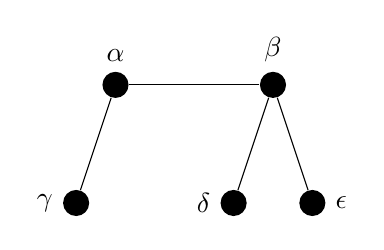
\begin{tikzpicture}
\node [label=above:{$\beta$}, fill=black, circle] (v2) at (-2,1) {};
\node [label=above:{$\alpha$},fill=black, circle] (v1) at (-4,1) {};
\node [label=left:{$\gamma$},fill=black, circle] (v3) at (-4.5,-0.5) {};
\node [label=left:{$\delta$}, fill=black, circle] (v4) at (-2.5,-0.5) {};
\node [label=right:{$\epsilon$}, fill=black, circle] (v5) at (-1.5,-0.5) {};
\draw  (v1) edge (v2);
\draw  (v1) edge (v3);
\draw  (v2) edge (v4);
\draw  (v2) edge (v5);
\end{tikzpicture}